\chapter[Automatically Generating TPNs]{Automatically Generating Temporal Planning Networks}
\label{chap: generating TPNS}

\paragraph{}Now that we have supplied the relevant motivation and background for the task at hand, we can further define the problem which we wish to solve. 

\section{Formal Problem Definition}
\label{generating: formal prob def}


\begin{tcolorbox}[colback=gray!5!white,colframe=gray!75!black]
\textit{Given a Temporal Planning task $\Pi = \langle F,A,I,G \rangle $ as input, we wish to generate a Temporal Planning Network (TPN) which represents multiple dissimilar plans that solve the task at hand.}
\end{tcolorbox}


\paragraph{Informally} we do not just want any TPN. We wish to generate a "good" TPN. 
As no current methods for comparing TPNs exist, we chose in this work to focus on generating 
the most compact TPN representation possible. To achieve this we will maximize the number of 
points our process merges along the obtained diverse plans.

While we are aware that other TPN attributes are also comparison-worthy, we advocate that smaller TPNs encode all the original plans compactly, reduce complexity by lowering the number of elements in the TPN and intuitively, are easier to communicate to a human counterpart. In addition, this objective steers towards a solution that requires more merges between the diverse plans, meaning more connections between them and as a result more flexibility during execution.

\paragraph{}
We note here that our work focuses primarily on the TPN time points $\mathcal{E}$ as these are the elements we wish to minimize in order to achieve the smallest TPN.

Merging time points often leads to new decision variables being generated. Different combinations of such decisions might lead to valid or invalid plans, thus, other possible optimization objectives could include generating TPNs with a high number of decision variable combinations, or which lead to a high number of valid plans. We leave optimizing these measures for future work.

Additionally, Pike (the TPN executive) incorporates the ability to avoid making combinations of choices that lead to infeasible paths and so we do not trouble ourselves with addressing how these merges may affect the TPN constraints $C$.

\paragraph{}We are now ready to start getting our hands dirty and describe how we tackle this problem. 
\section{Methods}
\label{generating: methods}


\paragraph{}First off, we describe our devised approach to Diverse Temporal Planning.
\subsection{Diverse Temporal Planning}
\label{background: Diverse Temporal}

Our approach to diverse temporal planning builds upon the top-$k$ approach in \cite{katz2019reshaping} using a {\em plan forbidding reformulation} as in \cite{katz2018novel} . 

The top-$k$ approach defines metrics in order to measure how close plans are to the best subset of all known plans, while the forbidding reformulation constitutes a diverse planning algorithm that instead of modifying the planner, in order to find a dissimilar solution, modifies the planning task itself. The reformulation occurs after each iteration (after which a plan is found) and alters the planning task in such a way as to forbid the possibility of finding the same solution that was obtained in the previous iteration.
%%

The main challenge we address here is that temporal plans are not a sequence of instantaneous happenings (IHs), but rather a schedule, and thus the top-$k$ approach does not apply directly. Therefore, we first define the {\em temporal plan skeleton} of a solution to a temporal planning task.

\begin{definition}[\textbf{Temporal Plan Skeleton}]
Given a planning task $\Pi = \langle F,A,I,G \rangle$ and a solution $\tau$. 
The temporal plan skeleton (TPS) $\pi$ is the sequence of the IHs in $\tau$ (without their time stamps).
\end{definition}

In other words, by observing only the sequence of occurrences in a temporal planning schedule, i.e. \textit{action-start} and \textit{action-end} events, we can refer to this TPS as a sequential plan for our diverse planning purposes. \\
We now define the \textit{TPS suffix} which will come in handy in section \ref{generating: merging} when choosing time-points for merging.

\begin{definition}[\textbf{TPS Suffix}]
Given a TPS $\pi$ and an IH $a \in \pi$. The TPS suffix of $\pi$ from $a$, denoted $\Sigma^\pi_a$, is the ordered sequence of IHs in $\pi$ from right after $a$ occurs (excluding $a$) until the end of the TPS.
\end{definition}


The objective of diverse temporal planning is to find dissimilar solutions to the temporal planning task $\Pi$. We argue that two different plans, with the same TPS, and which vary only in their time stamps, are not very different. Specifically, for the purposes of merging these plans into a TPN, they are not different at all, as the TPN executive will make the scheduling decisions. Thus, we define two plans to be different if and only if they have a different TPSs.

The diverse top-$k$ planning approach \cite{katz2019reshaping} works iteratively by calling a planner to obtain a solution $\tau$, then creating a modified planning task which eliminates the solution $\tau$, calling the planner again, and so forth.
Thus, to apply this approach to temporal planning, we create a {\em temporal plan elimination formulation}, which takes as input a temporal planning task $\Pi$ and a solution $\tau$, and creates a modified temporal planning task $\Pi'$ which eliminates all solutions which share the same TPS as $\tau$ (while all other solutions remain valid).

The main technical challenge here is that temporal planning is performed with durative actions, while the {\em plan forbidding reformulation} \cite{katz2018novel} works on IHs (as in classical planning). Furthermore, the plan forbidding reformulation is based on detecting when the current candidate plan deviates from the plan to forbid, which is simpler for classical planning. 

To overcome this challenge, we think of each durative action $a$ as two IHs; $a_{\vdash}$ at the start and $a_{\dashv}$ at the end. Note that a TPS is determined by the order of the IHs, similarly to a classical plan. 
Thus, if we could somehow plan with IHs (while still respecting action durations, invariant conditions, and temporal constraints) we could use the classical planning approach directly.
While this is not possible, we can think of a durative action as a pair of two IHs, and look at five different points where a durative action might deviate from the given TPS $\pi$. These are illustrated in Figure \ref{fig:compilation}, and correspond to the five cases described below.

\begin{figure}
\centering
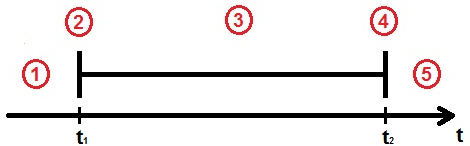
\includegraphics[width=0.6\textwidth]{graphics/compilation.jpg}
\caption{All the possible points to deviate from TPS $\pi$, from the point of view of the $i^{th}$ action in $\pi$, $a_i$.} \label{fig:compilation}
\end{figure}

\begin{description}
\item[\textbf{Case 1:}] We have already deviated from $\pi$ before $a$ started. 
\item[\textbf{Case 2:}] We followed $\pi$ until now, but action $a$ is different than the $i^{th}$ action in $\pi$.
\item[\textbf{Case 3:}] Action $a$ starts according to $\pi$, but between $a_{\vdash}$ and  $a_{\dashv}$, another instantaneous event occurs, which deviates from $\pi$.
\item[\textbf{Case 4:}] Action $a$ starts according to $\pi$, but the end event $a_{\dashv}$ is not according to $\pi$, i.e., the end event is not according to the sequence. This occurs when some other event should have occurred before $a_{\dashv}$.
\item[\textbf{Case 5:}] Action $a$ starts and ends according to $\pi$. This case is when $\pi$ is being followed, and a future action will deviate.
\end{description}

Having described these 5 cases, we can now describe our {\em temporal plan elimination formulation}. This formulation has 6 different versions of each durative action that takes part in the plan: one for each of the above five cases, and one for actions which do not appear in $\pi$. Also, similarly to the top-$k$ approach \cite{katz2018novel}, we introduce new proposition to encode deviation from $\pi$. Specifically, for a given TPS with $n$ IHs, we use $2n+2$ propositions: $2n+1$ to encode the sequence $\pi$, and another for representing whether we have already deviated. Note, that only durative action participating in the plan to forbid will be multiplied, and not the entire space of durative actions.

We now formally describe our formulation. Let $\Pi = \langle F,A,I,G \rangle$ be a planning task, and $\tau = \langle a_1, t_1, d_1\rangle ,...,\langle a_n, t_n, d_n\rangle$ be some temporal plan with a corresponding TPS $\pi$, where $i$ and $i'$ are the time indexes of $a_{\vdash}$ and $a_{\dashv}$ appropriately in $\pi$. The planning task $\Pi' = \langle F', A', I', G'\rangle$ is defined as follows:
% \begin{figure}[h]
% \centering
% \includegraphics[width=0.5\textwidth]{formulation.png}
% \end{figure}

\begin{itemize}
\item $F' = F \cup \{ p, p_0,..., p_{2n}\}$,
\item $A' = \{a^0 \ |\ a \in A, a \not\in \tau \} \cup  \{a^1,a^2,a^3,a^4,a^5 \ |\ a \in \tau \}$  \\
where:
\begin{align*}
a^0 = & \langle \text{pre}_{\vdash}(a), \text{eff}_{\vdash}(a) \cup \{p\} ,\text{inv}(a), \text{pre}_{\dashv}(a), \text{eff}_{\dashv}(a)\rangle\\ 
%
a^1 = & \langle \text{pre}_{\vdash}(a) \cup \{p\} , \text{eff}_{\vdash}(a), \text{inv}(a), \text{pre}_{\dashv}(a), \text{eff}_{\dashv}(a)\rangle\\
%
a^2 = & \langle \text{pre}_{\vdash}(a) \cup \{\neg p, \neg p_{i-1}\}, \text{eff}_{\vdash}(a) \land p, \text{inv}(a), 
 \text{pre}_{\dashv}(a),\text{eff}_{\dashv}(a)\rangle\\
%
a^3 = & \langle \text{pre}_{\vdash}(a) \cup \{\neg p, p_{i-1}\}, \text{eff}_{\vdash}(a) \land \neg p_{i-1} \land p_i, \text{inv}(a), \text{pre}_{\dashv}(a) \cup \{p\}, \text{eff}_{\dashv}(a)\rangle \\
%
a^4 =  & \langle \text{pre}_{\vdash}(a) \cup \{\neg p, p_{i-1}\}, \text{eff}_{\vdash}(a) \land p_{i-1} \land p_i, \text{inv}(a), \text{pre}_{\dashv}(a) \cup \{\neg p, \neg p_{i'-1}\}, \\ 
& \text{eff}_{\dashv}(a) \land p \rangle \\
%
a^5 = & \langle \text{pre}_{\vdash}(a) \cup \{\neg p, p_{i-1}\}, \text{eff}_{\vdash}(a) \land \neg p_{i-1} \land p_i, \text{inv}(a), \text{pre}_{\dashv}(a) \cup \{\neg p, p_{i'-1}\}, \\
&\text{eff}_{\dashv}(a) \land \neg p_{i'-1} \land p_{i'} \rangle
\end{align*}
\item $I' = I \cup \{p_0\}$
\item $G' = G \cup \{p\}$
\end{itemize}

\paragraph{Explaining the reformulation} For ease of presentation, we abuse notation and say that a temporal action $a$ is along $\pi$, when $a_{\vdash},a_{\dashv} \in \pi$ with indexes $i, i'$.
The variable $p$ represents a deviation from $\pi$, so it starts as false, and becomes true when the sequence of actions applied is not a prefix of $\pi$. Once the value $p$ is achieved, it remains true. $p$ is also part of the new goal, $G'$, as the objective here is to find a deviation from $\pi$.

Propositions $p_0, ..., p_{2n}$ encode the progress along the TPS $\pi$, before deviating from it. 
Actions $a^0$ are the activities that do not appear in $\pi$, thus automatically indicate deviation from $\pi$ and achieve $p$.
The actions $a^1, ..., a^4$ are copies of actions in $\pi$, 
corresponding to cases $1...4$ above. 
%for the cases when $\pi$ is already been discarded from consideration, and  $\bar p$ has been achieved, according to the cases described before. 
$a^5$ are copies of actions along $\pi$, these actions are responsible for following the sequence $\pi$ and are applicable only while the sequence is still followed, i.e. $p$ is false. Note that in all five cases when an action along $\pi$ has more than one instance, each instance is treated as a different action with a different corresponding $p_i$ variable indicating its position in the sequence. The convention in the reformulation is that the preconditions are sets which requirements are added to, and effects are sets comprised of delete and add effects, thus the conjunction between delete and add effects of the auxiliary variables.
% \footnote{The following theorem and an example will be made available during rebuttal if requested (as per the FAQ), and will be available in the final version of the paper with extra pages purchased.}

\begin{theorem}
Let $\Pi$ be a temporal planning task and $\tau$ a solution with TPS $\pi$. The task $\Pi'$ is a plan elimination reformulation of $\Pi$ and $\pi$.
\end{theorem}
Running the plan elimination reformulation on our input temporal planning task iteratively will yield the diverse solutions we desire.



\paragraph{}With a set of diverse TPSs $\{\pi_1 \ldots \pi_k\}$ at hand for our input planning task $\Pi$, we can dive in to tackling how to merge these into a single TPN representation, that compactly encodes all generated solutions and possibly more.
\subsection{Merging Diverse Plans into a TPN}
\label{generating: merging}
A naive merging approach for generating a TPN would be to create a single decision variable $v \in V$ corresponding to a choice 
between the $k$ obtained solutions. 
The structure of the TPN would then be a single decision at the
initial state, which is shared, and then the $k$ constituent plans running in parallel
up until they merge at the end of their path when reaching the terminal state which to is shared.
We denote this structure from now on as the \textit{naive TPN}. 
Although this approach defeats the purpose of having a flexible plan with choices, we would like to emphasize 
the fact that the naive TPN is attainable for any set of $k$ solutions. This means that no matter how big $k$ is 
or the length of each solution, we can always generate a functioning TPN to pass onward to Pike.
This by itself is already good news and provides our process with a degree of safety as a first step. 
    
The technique we describe here starts with the aforementioned naive TPN, but then looks for opportunities to merge additional time points.
It is convenient to think of a TPN as a graph where time points are nodes connected by constraints (edges).
By merging time points, additional solutions can be created, as demonstrated by the example in Figure \ref{fig:add_plans_from_merge}.

%\vspace{-1em}
\begin{figure}%[H]
    \centering
    \begin{minipage}[t]{0.5\textwidth}  \centering
        \begin{tikzpicture}[thick,scale=0.9, every node/.style={transform shape}]
            % x node set with absolute coordinates
            \node[state, accepting] (a) at (0,-1) {$I$};
            \node[state] (b) at (1,0) {$e^1_s$};
            \node[state] (c) at (3,0) {$e^1_f$};
            \node[state] (d) at (4.5,0) {$e^1_s$};
            \node[state] (e) at (6.5,0) {$e^1_f$};
            \node[state] (f) at (1,-2) {$e^2_s$};
            \node[state] (g) at (3,-2) {$e^2_f$};
            \node[state] (h) at (4.5,-2) {$e^2_s$};  
            \node[state] (i) at (6.5,-2) {$e^2_f$};
            \node[state, accepting] (j) at (7.5,-1) {$G$};
            % Directed edge
            \draw (a) edge (b);
            \draw (b) edge node[pos=0.5, sloped, above] {$Walk$} (c);
            \draw (c) edge  (d);
            \draw (d) edge node {$Order$} (e);
            \draw (a) edge  (f);
            \draw (f) edge node[pos=0.5, sloped, above] {$Taxi$} (g);
            \draw (g) edge  (h);
            \draw (h) edge node {$Cook$} (i);
            \draw (i) edge (j);
            \draw (e) edge (j);
        \end{tikzpicture}
    \end{minipage}
    \centerline {\rule{.8\linewidth}{1pt}}
    \begin{minipage}[t]{0.5\textwidth} \centering
        \begin{tikzpicture}[thick,scale=0.9, every node/.style={transform shape}]
            % x node set with absolute coordinates
            \node[state, accepting] (a) at (0,-1) {$I$};
            \node[state] (b) at (1,0) {$e^1_s$};
            \node[state] (d) at (4.5,0) {$e^1_s$};
            \node[state] (e) at (6.5,0) {$e^1_f$};
            \node[state] (f) at (1,-2) {$e^2_s$};
            \node[state] (h) at (4.5,-2) {$e^2_s$};  
            \node[state] (i) at (6.5,-2) {$e^2_f$};
            \node[state, accepting] (m) at (3,-1) {$e^1_f,e^2_f$};
            \node[state, accepting] (j) at (7.5,-1) {$G$};
            % Directed edge
            \draw (a) edge (b);
            \draw (b) edge node[pos=0.5, sloped, above] {$Walk$} (m);
            \draw (m) edge  (d);
            \draw (d) edge node[pos=0.5, sloped, above] {$Order$} (e);
            \draw (a) edge  (f);
            \draw (f) edge node[pos=0.5, sloped, above] {$Taxi$} (m);
            \draw (m) edge  (h);
            \draw (h) edge node[pos=0.5, sloped, above] {$Cook$} (i);
            \draw (i) edge (j);
            \draw (e) edge (j);
        \end{tikzpicture}
    \end{minipage}
    \caption{Additional paths in the graph are created as a result of a merge. Choice time points are depicted with double circles.\\
    \textbf{Top:} Two separate plans, number of possible paths: 2. \\
    \textbf{Bottom:} Two merged plans, number of possible paths: 4.}
    \label{fig:add_plans_from_merge}
    \vspace{-4mm}
\end{figure}


\begin{tcolorbox}[colback=red!5!white,colframe=red!75!black]
  \textit{Returning to our running example, let us consider the case where our robot, Rob, has conceived two constituent plans
   shown in a \textit{naive} TPN fashion at the top of Figure \ref{fig:add_plans_from_merge}.
   The plans are: $i$) walk home and then order in, or $ii$) take a taxi home and then cook.
   By merging a time point between the two paths, we obtain a new TPN, as portrayed in the lower section of the Figure, which yields 2 
   new solutions: walking home and then cooking, and taking a taxi home and then ordering in.
  }
\end{tcolorbox}


We next describe how we choose which time points from the naive TPN to merge.


\subsubsection{Merging Time Points in the TPN} 
While it is theoretically possible to merge any two time points in the TPN, it is likely a bad idea to merge two random time points. 

Some intuitive approaches include \textit{i)} comparing the underlying PDDL states of time points and \textit{ii)} comparing ordered sequences of activities originating from time points.
Unfortunately, both techniques fall short of accounting for important merges possibilities we wish to obtain. We showcase one of these approaches bellow:\\
\\
\textbf{State Space Comparison:} This approach imposes that for two time points to be merged, they must hold the same set of fact literals $F$. Although this constraint does ensure that time points that are chosen for merge can indeed be merged, it is too restrictive.\\
\begin{tcolorbox}[colback=red!5!white,colframe=red!75!black]
  \textit{Consider the merge witnessed in Figure \ref{fig:add_plans_from_merge}. The time points merged denoted the end of the activities whose purpose was to get Rob home. Once home, we can assume that the underlying PDDL states of $e^1_f$ and $e^2_f$ are similar and therefore this merge is plausible.\\
  Now consider a similar scenario with one key difference --- there exists a literal indicating the amount of money Rob has spent.
  Given that walking is free and a taxi costs money, we can expect that this state space comparison would rule out $e^1_f$ and $e^2_f$ as applicable for a merge.
    }
\end{tcolorbox}
This example shows how sensitive this method can be to the way each domain was constructed. 
Intuition would suggest that the solution to this issue is in locating the minimal set of literals that are of importance and only comparing those instead of all. This adjustment would work however the domain independent nature of automated planning makes finding this set of literals a nontrivial problem.
\\ \\
Thus we suggest a method to determine whether two time points should be merged based on the validity of the solutions originating from their merge.
We introduce the {\em compatibility} attribute of two IHs. We define compatibility based on IHs as opposed to time points as the latter can change when merging time points in the TPN while the former remains a static property of the TPSs of the original diverse solutions.
We define two notions of compatibility:
\begin{definition}[\textbf{IHs Compatibility}]
Given a pair of IHs $a_1,a_2$ from TPSs $\pi_i,\pi_j$ respectively, 
let $s_{a_1},s_{a_2}$ be 
the underlying PDDL state after these IHs occurred in $\pi_i,\pi_j$, respectively, and let their corresponding TPS suffixes be $\Sigma^{\pi_i}_{a_1}, \Sigma^{\pi_j}_{a_2}$.
$a_1,a_2$ are:
\begin{itemize}
    \item \textbf{Fully compatible} iff $G \subseteq T(s_{a_1},\Sigma^{\pi_j}_{a_2}) \; and \; G \subseteq T(s_{a_2},\Sigma^{\pi_i}_{a_1})$
    \item  \textbf{Semi compatible} iff $G \subseteq T(s_{a_1},\Sigma^{\pi_j}_{a_2}) \;  or \;  G \subseteq T(s_{a_2},\Sigma^{\pi_i}_{a_1})$
\end{itemize}
\end{definition}

In other words two IHs $a_1,a_2$ are Fully Compatible if we can execute the TPS suffix of each $\pi$ from the other's current state $s_a$ and achieve the goal, while two IHs $a_1,a_2$ are merely Semi Compatible if we can execute at least one of the TPS suffixes from the other's current state $s_a$ and achieve the goal.

We denote the set containing all such compatible pairs as $\MergeSet$. Since $\MergeSet$ is static, we can efficiently compute it once at the beginning of the process.
Each pair of compatible IHs $\{a_1,a_2\} \in \MergeSet$ is an operation $m$ corresponding to a merge we can perform on the TPN time points. 

From now on, we will restrict our attention to applying only merges between pairs contained in $\MergeSet$ to the TPN. While this limits the space of possible TPNs, it also reduces the complexity of the problem to a manageable size.
\\ \\  
Merging two time points in the TPN outputs a single new time point. This new time point must account for all IHs involved in the merge (recall that a time point may consist of multiple IHs). Therefore the merging of two time points is an operation between sets of IHs. Consider the 2-step merging sequence to the naive TPN $m(a_1,a_2),m(a_2,a_3)$. The first merge operation creates a new time point $e_{new}$. The second merge operation is now $m(e_{new},a_3)=m(\{a_1,a_2\},a_3)$.

This scenario raises questions about the compatibility attribute as it applies to sets of IHs. We can define different transitivity notions when merging in order to experiment with this concept and widen or narrow our solution space.
\begin{definition}[\textbf{Merge Transitivity}] 
    We define two notions of transitivity for when we allow merges to be made.
    Formally, a merge between time points $e_1,e_2$ is applicable iff:
    \begin{itemize}
        \item \textbf{Strict}: $\forall a_i \in e_1 \wedge \forall a_j \in e_2:   m\{a_i,a_j\} \in \MergeSet$ 
        \item \textbf{Loose}: $\exists a_i \in e_1 \wedge \exists a_j \in e_2: m\{a_i,a_j\} \in \MergeSet$
    \end{itemize}
\end{definition}

We have not limited ourselves to generating TPNs with only valid solutions as the TPN executive (Pike) incorporates the ability to avoid making combinations of choices that lead to infeasible paths \cite{levine2018watching}.



\paragraph{} Once $\MergeSet$ has been acquired, we require a method to determine which merge operations to execute. The reason for this necessity is that the merge operations in $\MergeSet$ are only compatible by definition in the naive TPN.
\subsection{Merge Selection}
\label{generating: merge selection}
Given a naive TPN and its corresponding $\MergeSet$, our algorithm must now decide which 
merge operations to initiate and at what order. 

\begin{tcolorbox}[colback=blue!5!white,colframe=blue!75!black]
     \textbf{Example:} Consider the following configuration --- the naive TPN contains three
     TPSs $\pi_1,\pi_2,\pi_3$ and there exist time points 
     $e_1, e_2, e_3$ in $\pi_1, \pi_2, \pi_3$, respectively, such that $e_1$ is fully
     compatible with $e_2$ \textit{or} $e_3$ but not with both (i.e $m(e_2,e_3) \not \in \MergeSet$).
     Therefore we must choose to either merge $e_1$ to $e_2$ or to merge $e_1$ to $e_3$.
  \end{tcolorbox}


The portrayed scenario demonstrates the dilemma we now face --- 
which pairs of time points to merge? 


%% CP
\subsubsection{Constraint Programming} To solve this optimization problem we call upon
CP to maximize the number of merges we can apply to the naive TPN and formulate the 
problem as a COP. \\ 

We define the set of all IHs participating in the optimization as $N$, in other words,
these are all the {\em different} IHs appearing in $\MergeSet$.
To mark a pair of IHs $a_i,a_j \in N$ as chosen to be merged together, 
we define the Boolean decision variable $m_{i,j}$. The set of all such variables is then
 $M \equiv \{m_{i,j} \mid \forall i,j \in N\}$.

Our objective is to create the smallest possible TPN, and this is done by merging {\em groups} of IHs. Thus, to formulate our optimization objective using the $m_{i,j}$ decision variables, we must create auxiliary decision variables for keeping track of groups. For example, merging $a_1, a_2$ and $a_3$ sets six decision variables to TRUE ($m_{1,2}, m_{2,1}, m_{1,3}, m_{3,1}, m_{2,3}$ and $m_{3,2})$, but only counts as one group.
To do so we assign each IH the shared minimal index $i$ of its group.
For example, given the group containing IHs $a_1,a_2,a_3$, each IH is assigned the shared minimal index $1$.
This assignment is described via an additional decision variable $s_i$ of type integer which is simply derived from the $m_{i,j}$ decision variables. The set of all such variables is then $S \equiv \{s_i \mid \forall i \in N\}$
The initial value for each shared minimal index variable is its own index: $s_i = i$.
The COP therefore contains $N^2 + N$ decision variables.

%% constraints
Let us now formulate the constraints applied in our COP.
These will also define the merging transitivity, as discussed previously, which we wish to apply to the TPN. 
The following constraints hold for both Strict and Loose configurations:
\begin{itemize}
    \item\textbf{Compatible Merges}:  $m_{i, j} \implies \{a_i, a_j\} \in \MergeSet$.
    \item \textbf{Symmetric Merges}:  $m_{i, j} \iff m_{j, i}$.
    \item \textbf{Shared Minimum Node}:  $s_i \neq i \implies m_{i, s_i} \;$ and\\
    $m_{i, j} \implies s_i = min(s_i, s_j)$
\end{itemize}

The Strict configuration contains a single additional constraint dictating that any merging between three time points must uphold that they are all compatible with one another:
 $m_{i, j} \wedge m_{i, k} \implies \{a_i, a_j\},\{a_i, a_k\},\{a_j, a_k\} \in \MergeSet$.
    
The Loose configuration allows more freedom for applying merges but must make sure no two IHs originating from the same original solution are merged. Therefore, for this configuration, we pass $P$, a mapping from time points to original solutions, as input to the COP. Therefore, $P \equiv \{p_i \mid  i = 1,...,k \}$ where $k$ is the number of TPSs. The additional constraints are then:  
\textit{i)} $m_{i, j} \implies p_i \neq p_j$ \textit{ii)} $m_{i, j} \wedge m_{i, k} \implies p_j \neq p_k $ \textit{iii)} $ s_i = s_j \implies p_i \neq p_j$

% the objective
Lastly, the objective function of the COP is to maximize the number of elements in $S$ whose value differs from their index, in other words we want to count the number of IHs which were merged. Formally: 
$f = Max \sum_{i=0}^{N} \mathbbm{1} \;|\;s_i \neq i$


\paragraph{} \centering This concludes our TPN generating process.\\
\centering we now showcase it's empirical results.\\